\chapter{Avaliação}\label{ch:Avaliacao}

No âmbito científico, a avaliação de um determinado objeto de estudo busca, de modo geral, elucidar seu real impacto e influências sobre um determinando ambiente. O presente Capítulo apresenta os principais passos tomados para a avaliação do \acf{JS} desenvolvido pelo atual trabalho. Cada etapa influente para a efetiva avaliação do jogo desenvolvido é descrita nas demais seções. Desde modo, a \autoref{sec:Preparativos} descreve sobre os principais preparativos para a execução da pesquisa, a \autoref{sec:seg} fala sobre a segmentação da amostra, a \autoref{sec:pretes} apresenta os resultados alcançados na etapa de pré-teste, a \autoref{sec:tes} os resultados do teste, a \autoref{sec:postes} os resultados do pós-teste, a \autoref{sec:apreciar} descreve os resultados obtidos na etapa de apreciação e a \autoref{sec:compilar} compila todos os resultados, comparando-os ao final com demais trabalhos na área. 

\section{Preparativos}\label{sec:Preparativos}

A corrente pesquisa realiza a avaliação do jogo \textbf{Infância Segura}, de modo a verificar se o jogo em si é capaz de comprir com seus preceitos pré-estabelecidos. O principal preceito do jogo consiste na ideia de que o jogo é capaz de instruir crianças entre 5 (cinco) e 8 (oito) anos a reconhecerem eventos praticados (ou tentados) de violência sexual infantil. Para tal, se faz indispensável a busca por uma amostra de crianças (dentro da faixa etária estabelecida). O conselheiro tutelar Willians Odia e a assistente social Daniella Maragno prestaram seus conhecimentos para a corrente pesquisa, elencando possível cenários de atuação. O intercâmbio de ideias levou a Escola Municipal Pauline Parucker do município de Joinville do estado de \ac{SC}. Após algumas reuniões, a escola prestou seu parecer favorável, se prestando a servir de cenário para a execução da presente pesquisa. A diretora Rafaella e a supervisora Angela, são as principais agentes envolvidas no processo; processo esse, firmado oficialmente pela Declaração de Ciência e Concordância das Instituições Envolvidas (\autoref{chap:DIE}). 

A Escola Municipal Pauline Parucker, se dispos a ceder um total 112 (cento e doze) crianças para a presente pesquisa, dividas em 4 (quatro) turmas: 2º Ano C, 2º Ano D, 3º Ano C, 3º Ano D. As crianças das turmas citadas foram convidados a participar da pesquisa. Para as crianças interessadas em participar da pesquisa foram entregues dois termos, o Termo de Assentimento (\autoref{chap:TA}) e uma versão resumida do Termo de Consentimento Livre e Esclarecido (\autoref{chap:curto}). A versão resumida do Termo de Consentimento Livre e Esclarecido surge de modo a reduzir a quantidade de documentos físicos necessários, sem reduzir de fato, seus conteúdos, isso pois, a versão resumida apresenta um endereço que eletrônico que leva ao termo na integra. Após um período de duas semanas, 33 (trinta e três) documentos retornaram: 8 (oito) do 2º Ano C, 12 (doze) do 2º Ano D, 10 (dez) do 3º Ano C e 3 (três) do 3º Ano D. Salienta-se que durante esse período, um vídeo explicativo sobre a pesquisa foi enviando pela escola (via \textit{WhatsApp}) aos guardiões legais das crianças. Por fim, enfatiza-se que todos os termos e protocolos foram publicados na Plataforma Brasil, os quais foram validados e aprovados pelo Comitê de Ética, sob o \ac{CAAE} nº 43602921.2.0000.0118.

%As crianças, em suas salas de aula e em horário escolar, são apresentadas à pesquisa. Após uma breve apresentação, os menores são convidados a participar da pesquisa. Para as crianças interessadas em participar da pesquisa são entregues duas vias de dois termos. Os termos entregues são o Termo de Assentimento e o Termo de Consentimento Livre e Esclarecido. É requisitado que as crianças apresentem tais termos aos seus guardiões legais, devendo retornar uma das vias de cada um dos termos para a escola. Só participam da corrente pesquisa as crianças com toda a documentação legal devidamente atestada. Visando garantir a integridade das assinaturas e fugir de falsificações cada assinatura é comparada ao documento de matrícula escolar assinado na escola presencialmente pelos pais/responsáveis de cada criança. Todos os termos e declarações do presente estudo são impressos em duas vias. A presente pesquisa se compromete a manter guardada uma das vias por um período de 5 (cinco) anos, assim como todos os registros e resultados alcançados. O término da coleta de toda a documentação legal demarca o início do processo de segmentação da corrente pesquisa. 


\section{Segmentação}\label{sec:seg}

Ao total, 33 (trinta e três) crianças apresentaram toda a documentação necessária para sua participação na corrente pesquisa. Uma vez estabelecido a quantidade de indivíduo aptos a participar no correte estudo, iniciou-se o processo de segmentação da amostra. 

A amostra de indivíduos foi segmentada em dois grupos: Grupo Controle e Grupo Experimental. A segementação resultou em um grupo controle composto por 18 (dezoito) crianças e um grupo experimental composto por 15 (quize) crianças. A disposição detalhada dos grupos ficou da seguinte maneira: grupo controle com 8 (oito) crianças do 2º Ano C e 10 (dez) crianças do 3º Ano C e grupo experimental com 12 (doze) crianças do 2º Ano D e 3 (três) crianças do 3º Ano D.


\section{Pré-teste}\label{sec:pretes}

A etapa de pré-teste do atual trabalho foi realizada no dia 19 (dezenove) de outubro de 2021 às 13h30 (hora local). A etapa de pré-teste surge na presente pesquisa com o objetivo de identificar, a existência ou não, de diferenças significas entre o grupo controle e grupo experimental, no que diz respeito aos seus conhecimentos sobre abuso infantil. A medição dos conhecimentos das crianças é feita com auxílio do instrumento avaliativo \acf{CKAQ} adaptado ao português (\autoref{chap:traduzido}). 

A etapa de pré-teste ocorreu em dois momentos, inicialmente com as turmas do 3º (terceiro) Ano na biblioteca da escola e posteriomente com as turmas do 2º (segundo) Ano em uma sala de aula tradicional. O processo do pré-teste foi inteiramente realizado pelo presente autor com acompanhamento da supervisora Angela, sendo ela a responsável pela separação e remanegamento das turmas, conforme o regimento escolar. À todas as crianças foi entregue uma cópia impressa do \ac{CKAQ} adaptado ao português. Após a entrega, breves instruções sobre o conteúdo do questionário e sua forma de preenchimento foram passadas (\autoref{chap:teste}). %(semelhante ao \autoref{chap:teste}). Qualquer dúvida poderia ser respondia com a criança levantando a mão.

O questionário foi lindo em voz alta as crianças. O número da questão era lido, juntamente com sua figura representativa para situar as crianças sobre a pergunta corrente do questionário que deveria ser marcada. Uma questão por vez era lida e relida, fornecendo em seguida, uma janela de tempo para as crianças deliberarem e responderem a questão. Foram realizados gestos de positivo e negativo com as mãos, nos nomentos que as crianças eram indagadas se concordavam ou se discordavam (se elas achavam verdade ou se elas achavam mentira) a última questão lida.

O presente estudo não se dispôs a ceder material para o preenchimento do questionário (como lápis e borracha). As crianças participantes, utilizaram seus próprios materiais escolares para assinalar as questões do questionário. O processo como um todo contou com a participação de 31 (trinta e uma)  crianças e durou uma hora e trinta minutos, finalizando às 15h (hora local). Cada momento de aplicação teve duração de quarenta e cinco minutos, com duas crianças faltante do grupo controle (uma de cada turma). Ao término, as crianças retornaram a sua agenda escolar sem demais prejuízos. Por fim, os questionários foram recolhidos e levados para análise.

A análise dos dados do questionário visa compreender melhor o conhecimento de ambos os grupos no que tange os assuntos ministrados pelo questionário em si. Dentre as informações que podem ser coletados por essa análise, está a taxa de acerto por questão. A taxa de acerto por questão do grupo controle pode ser obeservada na \autoref{fig:barrasCon}.

\begin{figure}[htb]

    \caption{\label{fig:barrasCon}Gráfico de Barras da taxa de acerto por questão no pré-teste (grupo controle).}
    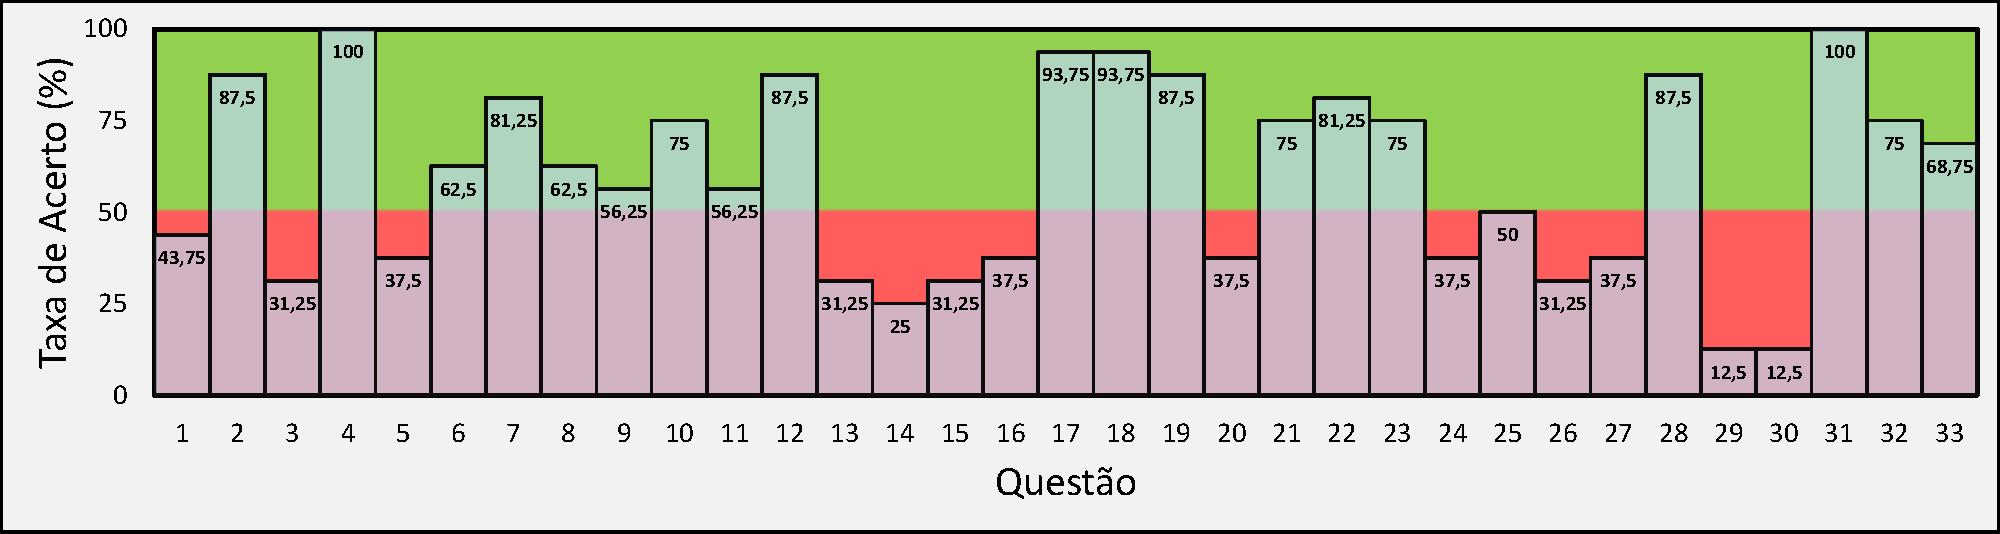
\includegraphics[width=\linewidth]{./Visuais/Notas4.pdf}
    \legend{Fonte: Elaborada pelo autor (2021).}
  
\end{figure}

A \autoref{fig:barrasCon} ilustra a taxa de acerto por questão (grupo controle). O eixo das abscissas representa cada uma das questões do questionário, sendo o número 1 (um) a primeira questão do questionário e o número 33 (trinta e três) a última questão do questionário. O eixo das ordenadas representa a taxa de acerto, indo de 0 (zero) a 100 (cem). O número 0 (zero) significa que nenhum indivíduo acertou aquela questão, o número 100 (cem) significa que aquela questão foi acertado por todos os indivíduos. No presente caso, tanto a questão 4 (quatro), quanto a questão 31 (trinta e um), tiveram uma taxa de acerto de 100\% para o grupo controle. O mesmo não ocorre com o grupo experimental como pode ser observado na \autoref{fig:barrasExp}.

\begin{figure}[htb]

    \caption{\label{fig:barrasExp}Gráfico de Barras da taxa de acerto por questão no pré-teste (grupo experimental).}
    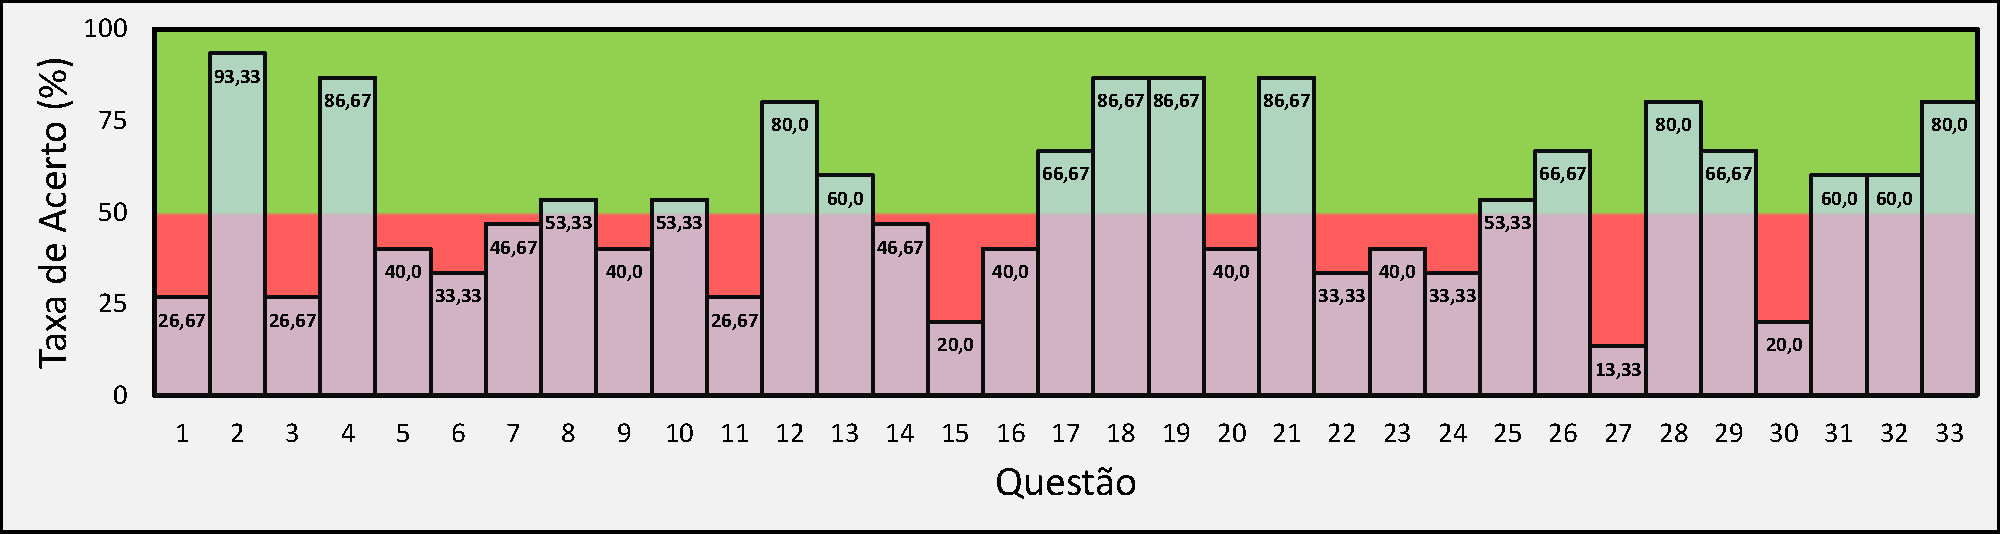
\includegraphics[width=\linewidth]{./Visuais/Notas3.pdf}
    \legend{Fonte: Elaborada pelo autor (2021).}
  
\end{figure}

A \autoref{fig:barrasExp} apresenta a taxa de acerto por questão (grupo experimental). Em comparação ao grupo controle (\autoref{fig:barrasCon}) o grupo experimental teve um desempenho ligeiramente inferior. Questões em branco ou rasuradas (de difícil identificação) foram consideradas erradas, ao total 26 (vinte e seis) questões estava rasuradas ou haviam sido deixadas em branco. Para fornecerem um panorama melhor da menor nota, maior nota e a média de cada grupo, produziu-se um diagrama de caixa estreita (\autoref{fig:caixapre}).


\begin{wrapfigure}[17]{r}{10.0cm}%pulando 17 linhas
    \vspace{-4pt}
    \caption{\label{fig:caixapre}Diagrama Caixa Estreita das notas (pré-teste).}
    \vspace{8pt}
    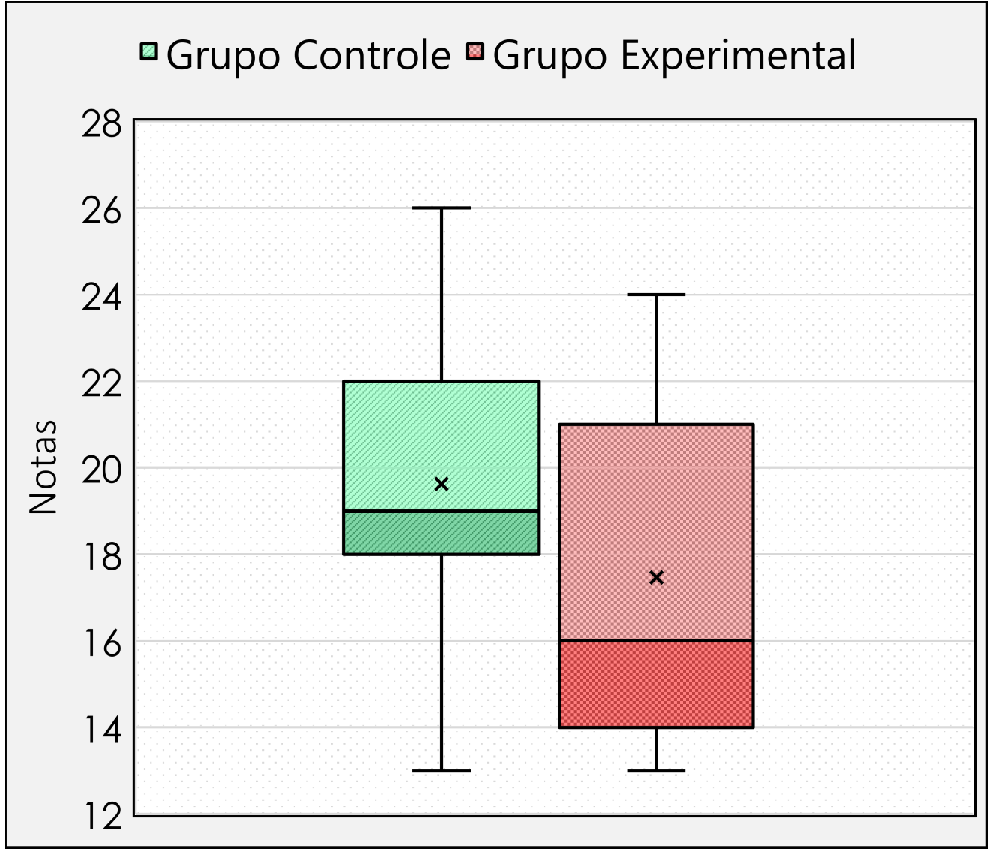
\includegraphics[width=\linewidth]{./Visuais/CaixaEstreitaEnfeitado.pdf}
    \legend{Fonte: Elaborada pelo autor (2021).}
\end{wrapfigure}

Um diagrama caixa estreita mostra a distribuição dos dados em quartis, realçando a média e as exceções. No caso do presente estudo o grupo controle acertou em média 19,625 ($\sigma$ = 3,18) questões (59,47\%, $\sigma$ = 9,64), enquanto o grupo experimental acertou em média 17,467 ($\sigma$ = 3,96) questões (52,93\%, $\sigma$ = 12), valores representados pela marcação em $\times$ na \autoref{fig:caixapre}. A maior quantidade de acertos foi de 26 (vinte e seis) questões no grupo controle e 24 (vinte e quatro) questões no grupo experimental. Ambos os grupos tiveram uma menor quantidade de acertos de 13 (treze) questões.

Para a devida condução da atual pesquisa é preciso garantir que as amostram sejam equivalentes entre si. Para averiguar o grau de equivalência entre duas amostras a estatística faz uso do Teste-T. Contudo, para se utilizar o Teste-T, é preciso determinar a priori, se a variância entre os grupos é igual ou diferente. Após os cálculos, os resultados indicaram que as  variâncias do grupo controle e grupo experimental são equivalentes ($\alpha$ = 0,05). Deste modo, o Teste-T foi realizado assumindo variância iguais entre as amostras, concluíndo ao final que as amostras são de fato, equivalentes ($\alpha$ = 0,05). A \autoref{fig:normal} ilustra a equivalência entre as amostras. 

\begin{figure}[htb]
    \centering
    \caption{\label{fig:normal}Distribuição das notas atingidas no pré-teste}
    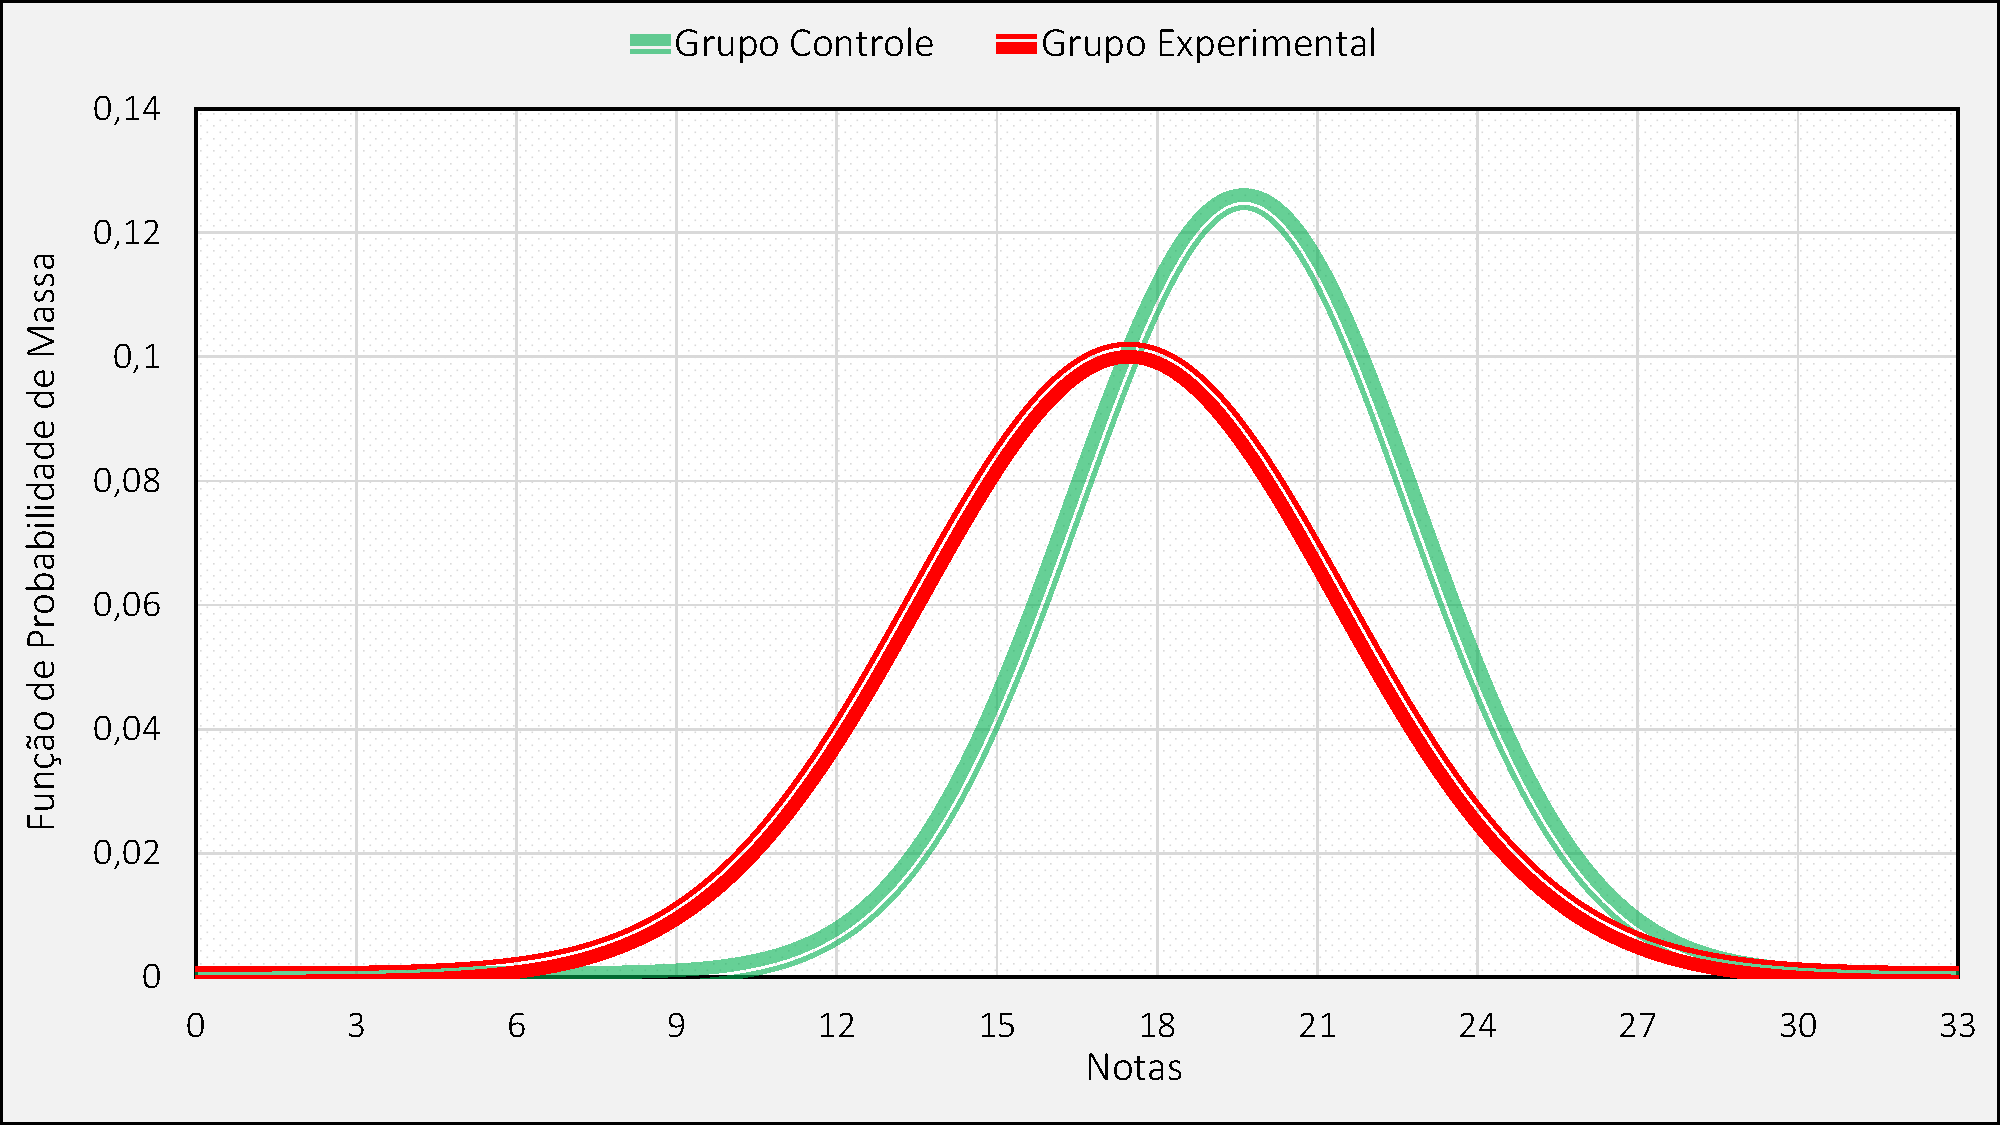
\includegraphics[width=\linewidth]{./Visuais/Graficos1.pdf}
    \legend{Fonte: Elaborada pelo autor (2021).}
  
\end{figure}


\section{Teste}\label{sec:tes}

A etapa de teste do atual trabalho ocorreu em três momentos distintos; dia 3 (três), dia 4 (quatro) e dia 5 (cinco) de novembro de 2021. No dia 3 (três) foram realizados os preparativos para a instalação do jogo nos \textit{tablets} da escola (modelo \textit{Multilaser} M10A). O processo se iniciou às 14h e terminou às 16h15 (hora local). O processo de instalação do jogo nos \textit{tablets} se deu na biblioteca da escola e contou com a participação da professora Carla Diacui Medeiros Berkenbrock, a suprevisora Angela e o presente autor desta dissertação. Ao total o jogo foi instalado em 30 (trinta) \textit{tablets}. Foi realizada a instalação do jogo em mais \textit{tablets} do que o necessário, visando contornar demais empecilhos como problemas ou falta de energia em algum determinado dispositivo durante a etapa de teste (apenas um \textit{tablets} foi trocado durante os experimentos). Ao final, todos os \textit{tablets} foram colocados em um gabinete de recarga.

Nos dias 4 (quatro) e 5 (cinco) de novembro de 2021 a presente pesquisa conduziu sua etapa de teste com crianças (na bilioteca da escola). O processo consistiu em submeter aos participantes (crianças), o objeto estudado (jogo). No dia 4 (quatro) as crianças participantes foram instruidas a jogar o jogo \textbf{Infância Segura}, mais especificamente as fases sobre \textbf{Direitos} (\autoref{subsec:2}) e \textbf{Denúncias} (\autoref{subsec:3}). No dia 5 (cinco) as crianças foram instruidas a jogar as demais fases, sobre \textbf{Anatomia} (\autoref{subsec:1}) e \textbf{Redes Sociais} (\autoref{subsec:4}). Essa separação das fases foi uma sugestão da suprevisora Angela. É importante salientar que a etapa de teste foi conduzida inteiramente e apenas com as crianças do grupo experimental, com uma criança do 3º Ano D faltante no dia 5 (cinco). Em ambos os dias o processo se iniciou às 13h40.

No dia 4 (quatro) e no dia 5 (cinco) os \textit{tablets} foram retirados do gabinete de recarga e distribuídos sobre as mesas da biblioteca da escola. As crianças foram entrando, duas a duas, na biblioteca da escola, sendo instruídas a sentarem na frente do \textit{tablet} que contivesse uma etiqueta com seu nome escrito (no último dia a posição dos \textit{tablets} foi trocada). Em ambos os dias as crianças tiveram contato com o jogo por quarenta e cinco minutos, totalizando ao total uma hora e trinta minutos de atividades (com início às 14h15 e término às 15h). O processo foi inteiramente conduzido pelo presente autor desta dissertação, com auxílio da suprevisora Angela (todos os dias). Em separado, no 4 (quatro) a professora Carla Diacui Medeiros Berkenbrock e no dia 5 (cinco) a aposentada Rocilda Cordeiro Mendonça, prestaram sua atenção e auxílio a pesquisa. Em específico a suprevisora Angela foi a responsável pelo remanejamento dos estudantes. %Em específico a suprevisora Angela foi a responsável por remanejar os estudantes das suas salas à biblioteca (e vice-versa).

No primeiro dia, as crianças foram apresentadas ao jogo com auxílio de um projetor. Neste momento as crianças foram instruídas a se identificarem no jogo e a informarem seu gênero. As crianças também foram instruídas a como alterar o volume do jogo e a como intercambiar entre as fases. No segundo dia, com auxílio do mesmo projetor, realizou-se uma revisão do terceiro minijogo da fase sobre \textbf{Direitos} e do primeiro minijogo da fase sobre \textbf{Redes Sociais}. Tais minijogos foram escolhidos para uma revisão, uma vez observado que os conteúdos contidos nestes minijogos coincidiam com os conteúdos das questões com menores taxas de acerto para o grupo experimental na etapa de pré-teste (\autoref{sec:pretes}).

No segundo dia, as crianças (em geral) apresentaram muita dificuldade para concluir o primeiro e o segundo minijogo da fase sobre \textbf{Anatomia}. Em virtude dessa dificuldade, instruções mais detalhadas de casa minijogos foram passadas com auxílio de um projetor. Por fim, a taxa de conclusão do jogo (quatro fases) ficou em 89,63\%. Ao todo 7 (sete) crianças deixaram de concluir uma ou mais fases no jogo. A escola e a internet foram as fases com melhor desempenho dos estudantes. Seguidos pela fase da delegacia e fase do hospital com os piores desemepnhos. 

No segundo dia havia instabilidade na internet da escola o que impossibilitou que os dados dos estudantes fossem enviados aos servidores. Pensando em falhas de conexão com o bando de dados, o jogo armazanava a todo mundo as ações dos seus jogadores localmente (nos tablets). Ao total 3315 ações nos minijogos foram computadas, dando em média 221,83 ações por jogador. Após o fim dos experimentos no segundo dia, o conteúdo de cada jogador foi extraido dos tablets(o processo levou em torno de uma hora). Por fim, a etiqueta dos tablet foi removida, os tablets foram desligados e colocados em um gabinete de recarga.

Durante a pesquisa alguns BUGS apareceram:
1-) na fase do hospital quando as crianças tocavam sem delicadeza nos tablet (varios toques, ou toques muito rapidos) a peça ficava travada, como no quebra-cabeça. 
2-) isso vale para a primeira e segunda fase do jogo do hospital.
Durante a pesquisa alguns BUGS apareceram: 
1-) Mapa travou em alguns (arrastar o mapa)
2-) Conectar os pinos tambem travou
3-) O quebra-cabeça travou
4-) Algumas mudaram o idioma do JOgo para Ingles/Espanhol

Algumas crianças tiveram dificuldade em colocar as peças e NÃO COMPREENDERAM O QUE DEVIA SER FEITO NA SEGUNDA FASE DO HOSPITAL. Elas não sabia que deviam marcar as partes intimas, e nem sabia quais partes deveriam marcar (jogo MUITO POUCO INTUITO).

Algumas crianças foram no banheiro.

É importante nenhuma das crianças que ojgaram o apresentam Daltonismo....  A falta de fone foi um fator triste (muito barulho atrapalhando as crianças).

Algums crianças pareciam responder o mais rapido possivel sem prestar atenção na pergunta. (talvez o tempo ser um fator de pontuação não seja legal.) 

Sugestões de melhorias deliberadas durante a etapa são tratadas na conclusão deste trabalho.


\section{Pós-teste}\label{sec:postes}


Praprado na escola 25 (vinte e cinco) de novembro de 2021

\section{Apreciação}\label{sec:apreciar}

Praprado na escola 25 (vinte e cinco) de novembro de 2021

\section{Compilação}\label{sec:compilar}

\subsection{Meus}\label{subsec:meus}


112 crianças (Turmas C e D, 2 e 3)
2C = 8 crianças
2D = 12 crianças
3C = 10 crianças
3D = 3 crianças


\subsection{Comparativo}\label{subsec:outros}

%\section{Considerações Finais}\label{sec:compilar}


*Resultados Finais

*Conclusão







A atual pesquisa submente o instrumento avaliativo \ac{CKAQ} para sua amostra de participantes (grupo controle e grupo experimental). A submissão do \ac{CKAQ} ocorre em duas etapas distintas da presente pesquisa, inicialmente na etapa de pré-teste e posteriormente na etapa de pós-teste. O instrumento avaliativo é entregue de maneira impressa e administrado verbalmente em sala de aula e em horário escolar para todos os participantes válidos de uma turma. Participantes inválidos (\textit{e.g.} crianças com participação não aprovada por seus guardiões legais) são direcionados para um atividade escolar sob responsabilidade da escola. Após a administração do \ac{CKAQ}, suas cópias impressas com as respostas dos participantes são colhidas e embaralhadas. Tal coleta encerra a etapa de pré-teste e demarca o início da etapa de teste da presente pesquisa.

%Tal versão é submetida ao grupo controle e ao grupo experimental em momentos distintos de maneira coletiva. O questionário é adminitrado verbalmente e as crianças devem responde-lo em suas folhas. Cada criança tem um indetificador. O questionário tem previsão de ser respondido em 15 minutos. Essa etapa consiste em colher a Aprendizagem (dado quantitativo) sobre  a temática de ambos os grupos. O questionário pode ser administrado por um dos pesquisadores ou por outro responsável optado pela escola. Ao término do questionário as folhas serão colhidas de cada participantes para análise. 


%Os resultados alcançados com o grupo estudado se demonstrar bem sólidos e robustos. Isso pois, a presente pesquisa se utiliza do Teste-t com um grau de confiança de 95\%. A alta taxa de confiança estatística do presente estudo, abre margem para uma defesa sólida e robusta de seus resultados. 

TESTES TESTES.....

Uma turma com 112 (cento e doze crianças) foram seleciondas para participantarem dessa pesquisa da Escola Municipal Pauline Parucker. Todos os protoclos foram segufios....









